\chapter{KẾT QUẢ}
\label{Chapter4}

% Trình bày kết quả: kết quả các kỹ thuật đã đạt được trên 
Chương \ref{Chapter4} đưa ra kết quả về việc hoạt động và các kỹ thuật triển khai trên phần cứng, \acrshort{vps}, và giao diện web.

\section{Kết quả trên phần cứng}

Kết quả trên phần cứng được trình bày, bao gồm kết quả hoạt động của kỹ thuật giao tiếp, đồng bộ, và mật mã hóa.

\subsection{Kỹ thuật giao tiếp}

Kỹ thuật giao tiếp được cài đặt như nhau trên \acrshort{mcu} STM32 và ESP32. Vì vậy, dựa trên log của \acrshort{mcu} ESP32, một giao tiếp với device và \acrfull{api} server điển hình (minh họa như hình \ref{fig:communication-of-device-server}) sẽ diễn ra trong khoảng $100ms\rightarrow 150ms$. Thống kê của 10 lần giao tiếp liên tiếp (minh họa như hình \ref{fig:10-measure-commu-physic}) cho thấy quá trình giao tiếp diễn ra trong khoảng $66.5ms$ và mã hóa/giải mã diễn ra trong $167\mu s$.

\begin{figure}[htp]
\centering
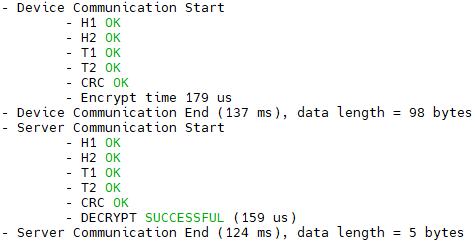
\includegraphics[width=1.0\linewidth]{images/fig-communication-of-device-server.png}
\caption{Một giao tiếp điển hình với device và server.}
\label{fig:communication-of-device-server}
\end{figure}

\begin{figure}[htp]
\centering
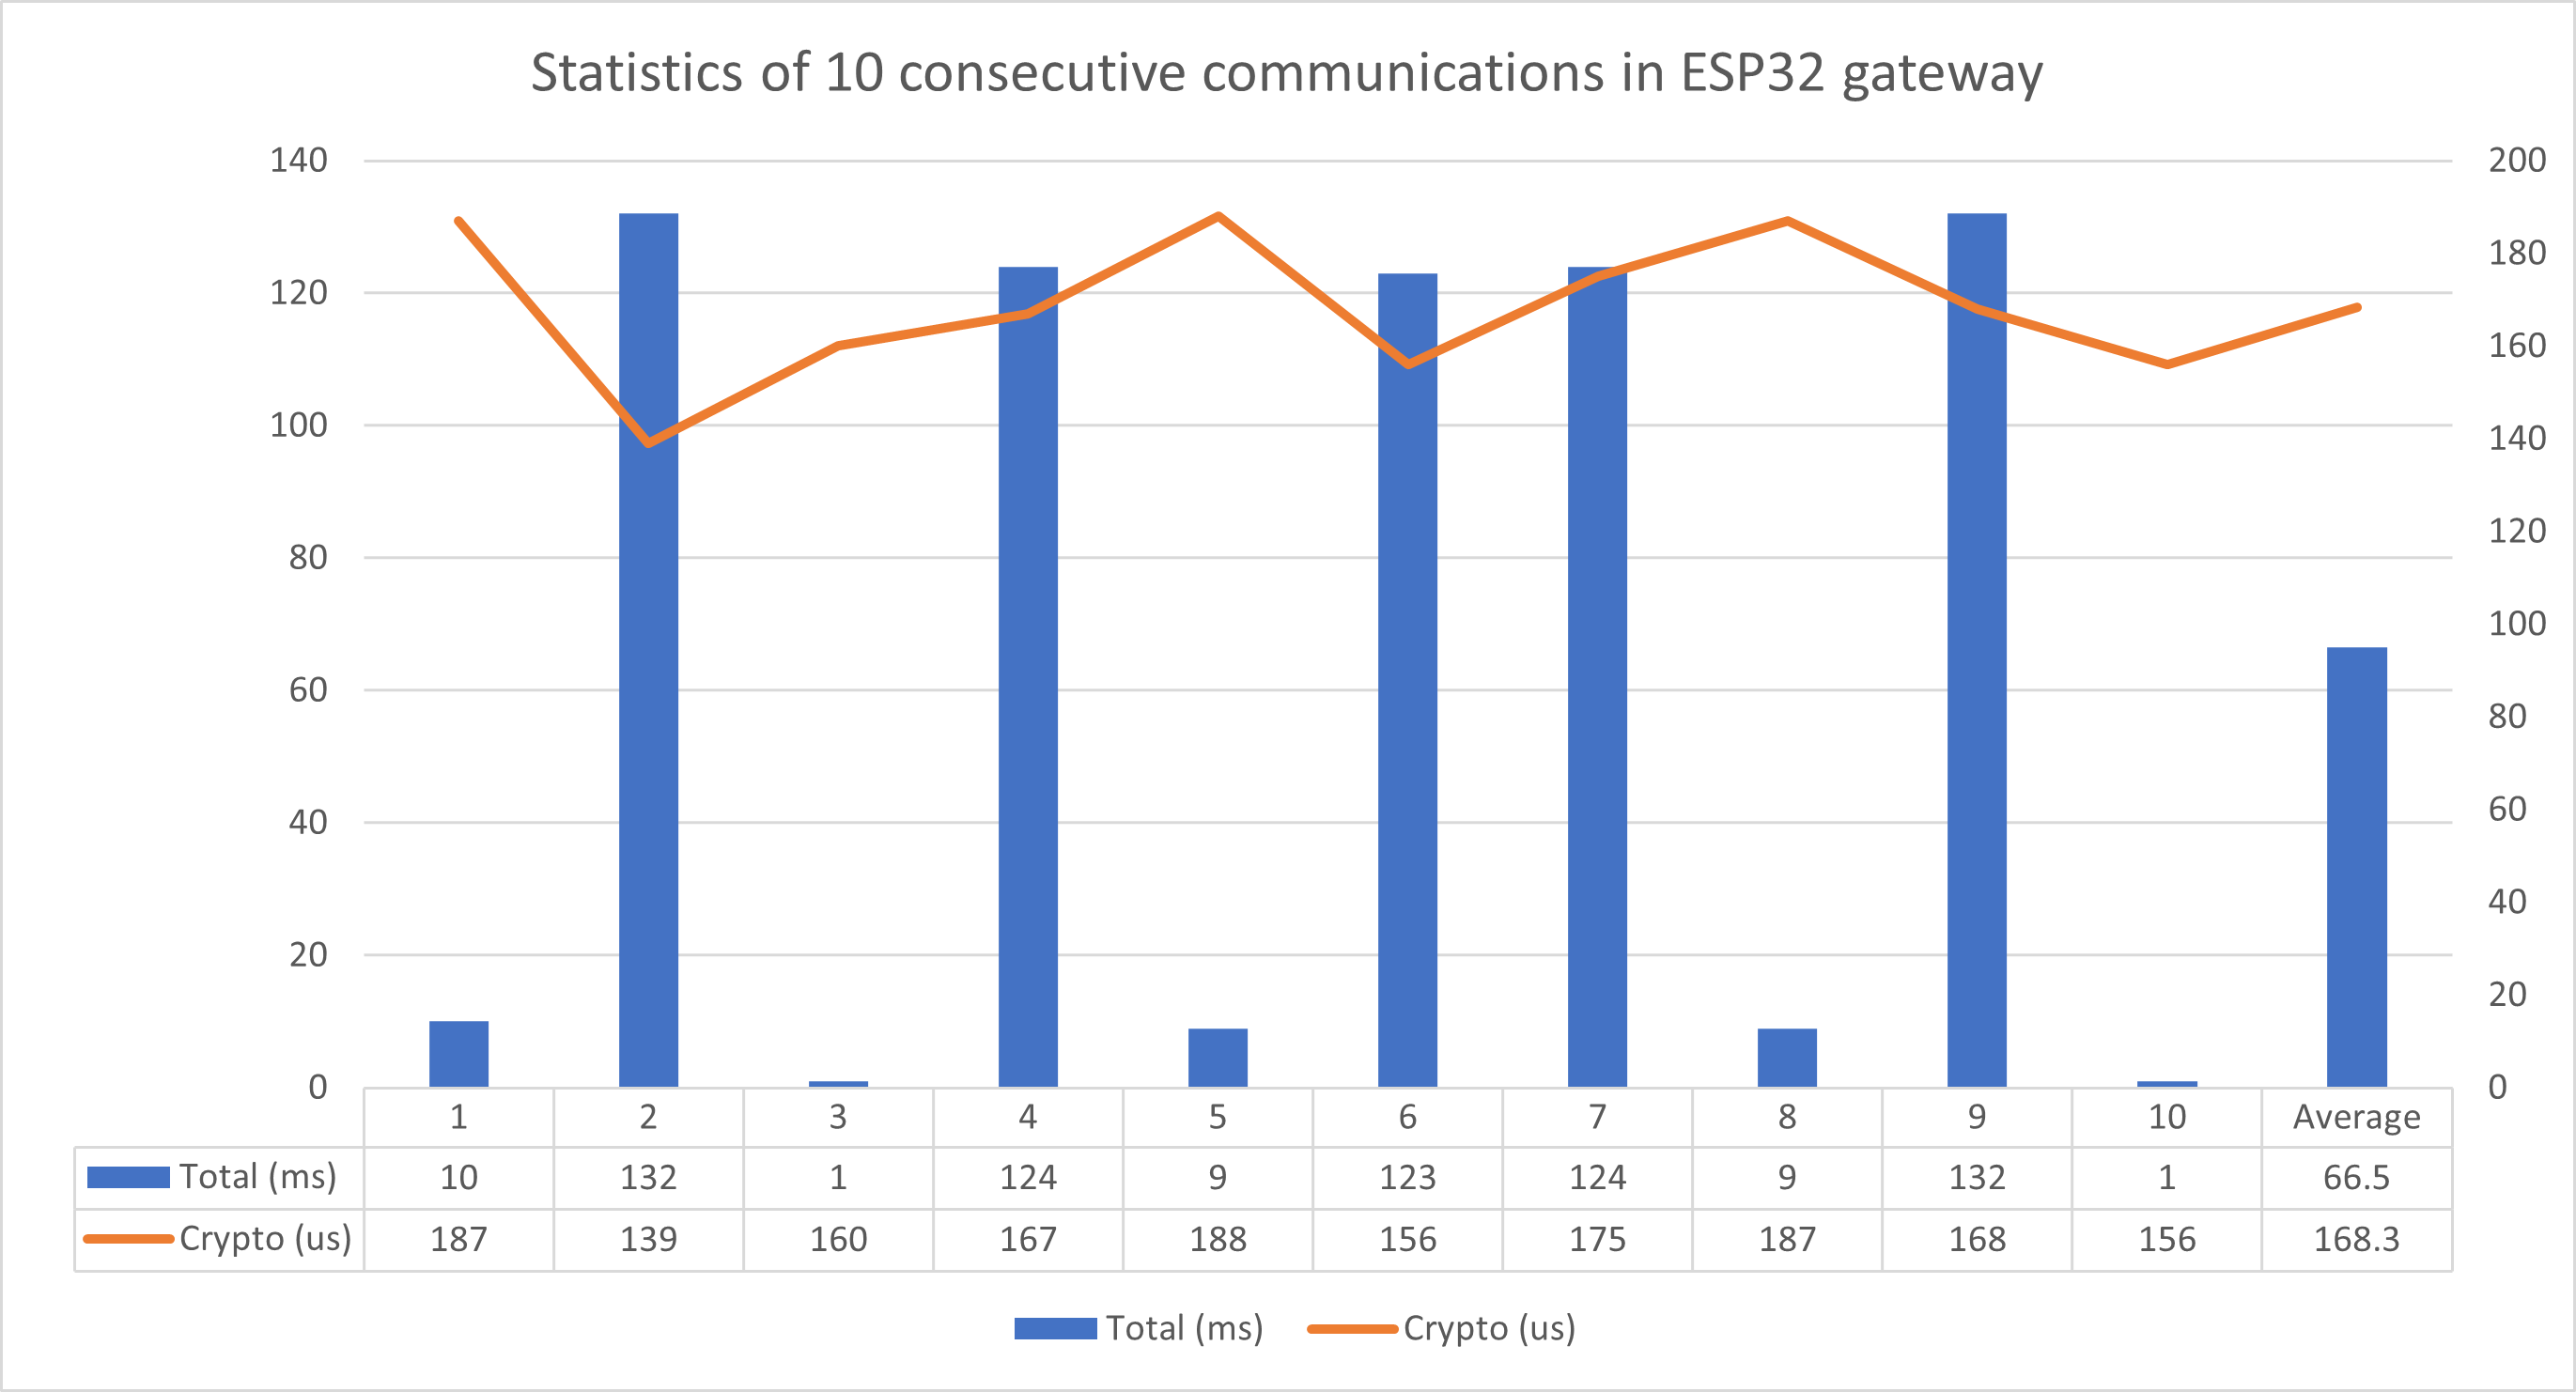
\includegraphics[width=1.0\linewidth]{images/fig-10-measure-commu-physic.png}
\caption{Thống kê của 10 quá trình giao tiếp liên tiếp.}
\label{fig:10-measure-commu-physic}
\end{figure}

\subsection{Kỹ thuật mật mã hóa}
% Minh họa quá trình thiết lập key CC20, onetime key Poly1305
Kỹ thuật mật mã hóa sử dụng thuật toán \acrshort{aead} ChaCha20-Poly1305 được triển khai thành công trên \acrshort{mcu} ESP32. Theo kiến trúc của thuật toán \acrshort{aead}, quá trình mã hóa (minh họa như hình \ref{fig:CC20-P1305-En-Process}) đã diễn ra đúng đắn và tuần tự theo các quá trình của RFC7539~\cite{rfc7539}:

\begin{enumerate}
    \item Thiết lập State cho Poly1305 one-time key.
    \item Tạo Poly1305 one-time key.
    \item Thực thi ChaCha20 encryption function.
    \item Thực thi Poly1305 function cho ciphertext.
\end{enumerate}

Và quá trình giải mã (minh họa như hình \ref{fig:CC20-P1305-De-Process}) đã diễn ra đúng đắn và tuần tự theo các quá trình của RFC7539~\cite{rfc7539}:

\begin{enumerate}
    \item Thiết lập State cho Poly1305 one-time key.
    \item Tạo Poly1305 one-time key.
    \item Thực thi Poly1305 function cho ciphertext.
    \item Thực thi ChaCha20 dencryption function.
\end{enumerate}

\begin{figure}[htp]
\centering
\captionsetup{justification=centering,margin=2cm}
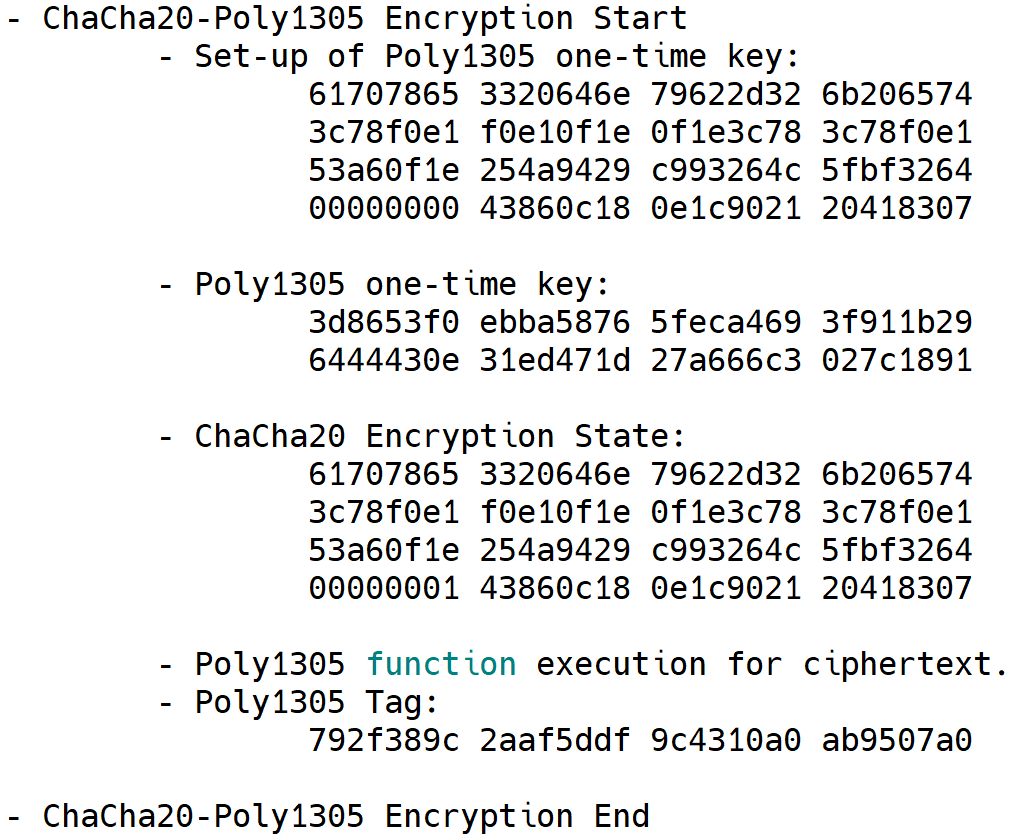
\includegraphics[width=0.7\linewidth, frame]{images/fig-CC20-P1305-En-Process.png}
\caption{Quá trình mã hóa của thuật toán \acrshort{aead} ChaCha20-Poly1305 trên \acrshort{mcu} ESP32.}
\label{fig:CC20-P1305-En-Process}
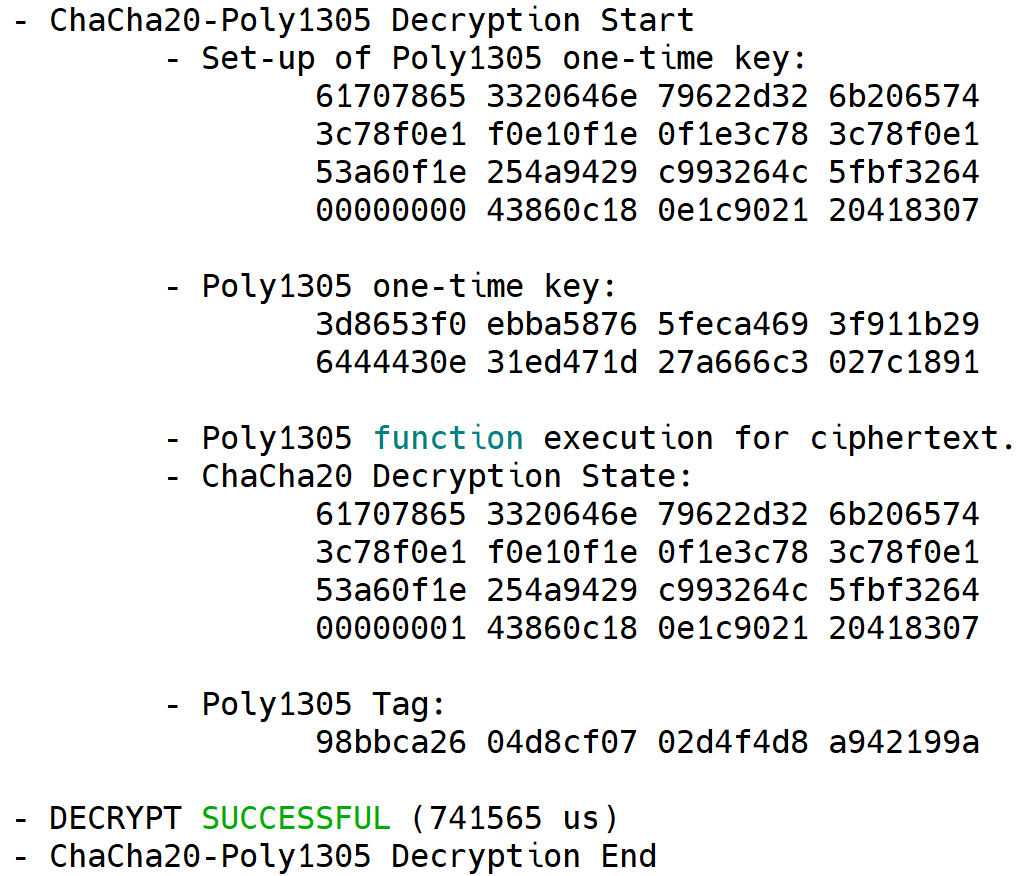
\includegraphics[width=0.7\linewidth, frame]{images/fig-CC20-P1305-De-Process.png}
\caption{Quá trình giải mã của thuật toán \acrshort{aead} ChaCha20-Poly1305 trên \acrshort{mcu} ESP32.}
\label{fig:CC20-P1305-De-Process}
\end{figure}

\subsection{Kỹ thuật đồng bộ}

Kỹ thuật đồng bộ được triển khai thành công trên firmware của \acrshort{mcu} STM32. Trên công cụ STM32CubeIDE, callback đồng bộ với \acrshort{vs}1 (minh họa như hình \ref{fig:VS1-callback-trig}) được thực hiện khi có sự thay đổi dữ liệu của \acrshort{vs} này trên database của \acrshort{vps}. Callback này được theo dõi thông qua breakpoint trên IDE.

\begin{figure}[htp]
\centering
\captionsetup{justification=centering}
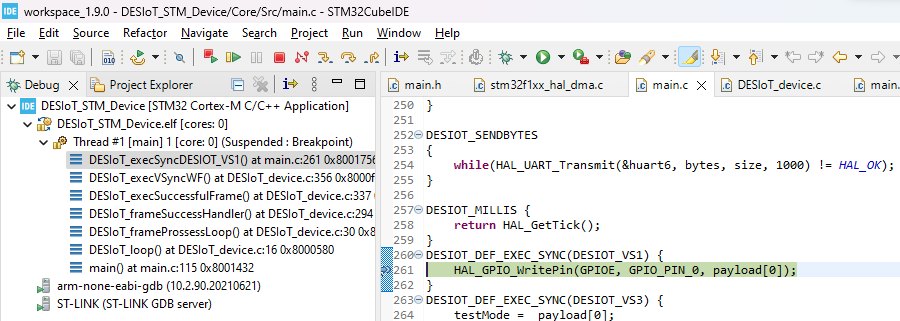
\includegraphics[width=1.0\linewidth, frame]{images/fig-VS1-callback-trig.png}
\caption{Breakpoint theo dõi callback đồng bộ với \acrshort{vs}1 được thực hiện trên STM32CubeIDE.}
\label{fig:VS1-callback-trig}
\end{figure}

\section{Kết quả trên VPS}

Trên \acrshort{vps}, các kết quả được minh họa bao gồm kết quả của kỹ thuật Docker Containerizing, Nginx web server, \acrshort{mqtt} Broker, MongoDB server, và các kết quả của giao tiếp và đồng bộ trên \acrshort{api} server.

\subsection{Kết quả của kỹ thuật Docker Containerizing}

Hệ thống back-end bao gồm \acrshort{mqtt} Broker, \acrshort{api} server, và MongoDB database, đã được triển khai thành công trên \acrshort{vps} thông qua kỹ thuật Docker Containerizing. Cụ thể, commandline của \acrshort{vps} khi chạy lệnh ``docker ps'' (minh họa như hình \ref{fig:docker-ps-vps}) hiển thị lần lượt các container của \acrshort{api} server, 3 replica set của MongoDB, và \acrshort{mqtt} Broker. Trong đó:

\begin{itemize}
    \item \acrshort{api} server chạy trên container \textbf{desiot-server-desiot-server-1} và hoạt động ở port 7001.
    \item Các replica set của MongoDB chạy trên các container \textbf{mongo1}, \textbf{mongo2}, và \textbf{mongo3} cũng như hoạt động ở các port $30001\rightarrow 30003$.
    \item \acrshort{mqtt} Broker chạy trên container \textbf{iot-services-broker-1} và hoạt động ở port 1883.
\end{itemize}

\begin{figure}[htp]
\centering
\captionsetup{justification=centering}
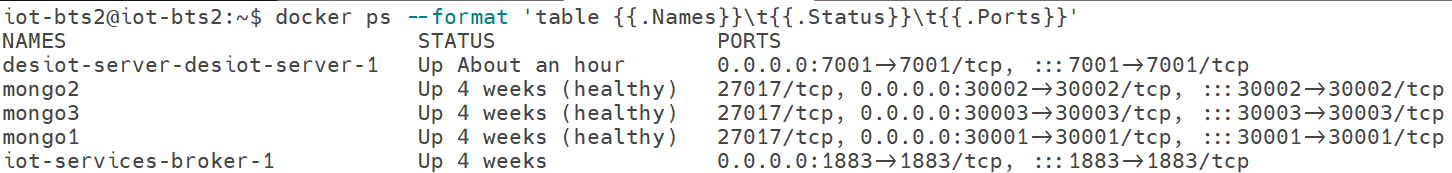
\includegraphics[width=1.0\linewidth, frame]{images/fig-docker-ps-vps.png}
\caption{Hệ thống back-end được triển khai trên \acrshort{vps}.}
\label{fig:docker-ps-vps}
\end{figure}

\subsection{Kết quả Nginx web server}

Nginx web server đã host thành công giao diện web của hệ thống \acrshort{iot}. Cụ thể, giao diện web được host tại địa chỉ \href{https://cloud.desiot.accesscam.org}{https://cloud.desiot.accesscam.org} và được cấp chứng chỉ SSL (minh họa như hình \ref{fig:ssl-cert}).

\begin{figure}[htp]
\centering
\captionsetup{justification=centering}
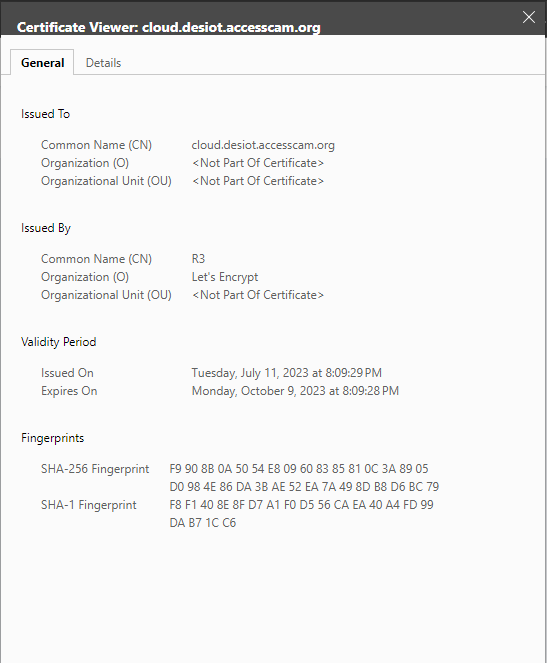
\includegraphics[width=0.6\linewidth, frame]{images/fig-ssl-cert.png}
\caption{Chứng chỉ SSL của giao diện web.}
\label{fig:ssl-cert}
\end{figure}

\subsection{Kết quả giao tiếp trên API server}

Trên \acrshort{api} server, quá trình phân giải và xử lý frame diễn ra khác với quá trình trên phần cứng. Cụ thể, trên \acrshort{api} server, quá trình này diễn ra trên một frame hoàn chỉnh thay vì trên từng byte rời rạc như quá trình trên các \acrshort{mcu}. Vì vậy, một quá trình phần giải và xử lý frame cụ thể trên \acrshort{api} server (minh họa như hình \ref{fig:frame-parsing-process-api-server}) sẽ xử lý đồng thời việc kiểm tra các header, trailer, và CRC. Sau đó, quá trình giải mã diễn ra. Thống kê của 10 lần giao tiếp liên tiếp với gateway (minh họa như hình \ref{fig:10-measure-commu-server}) có thời lượng giao tiếp trung bình với gateway diễn ra trong $15.5385ms$ cũng như thời gian giải mã trung bình là $9.9948\mu s$. Thời gian trung bình giao tiếp này nhanh hơn 4.2 lần so với gateway, và thời gian giải mã trung bình nhanh hơn 16.7 lần.

\begin{figure}[htp]
\centering
\captionsetup{justification=centering}
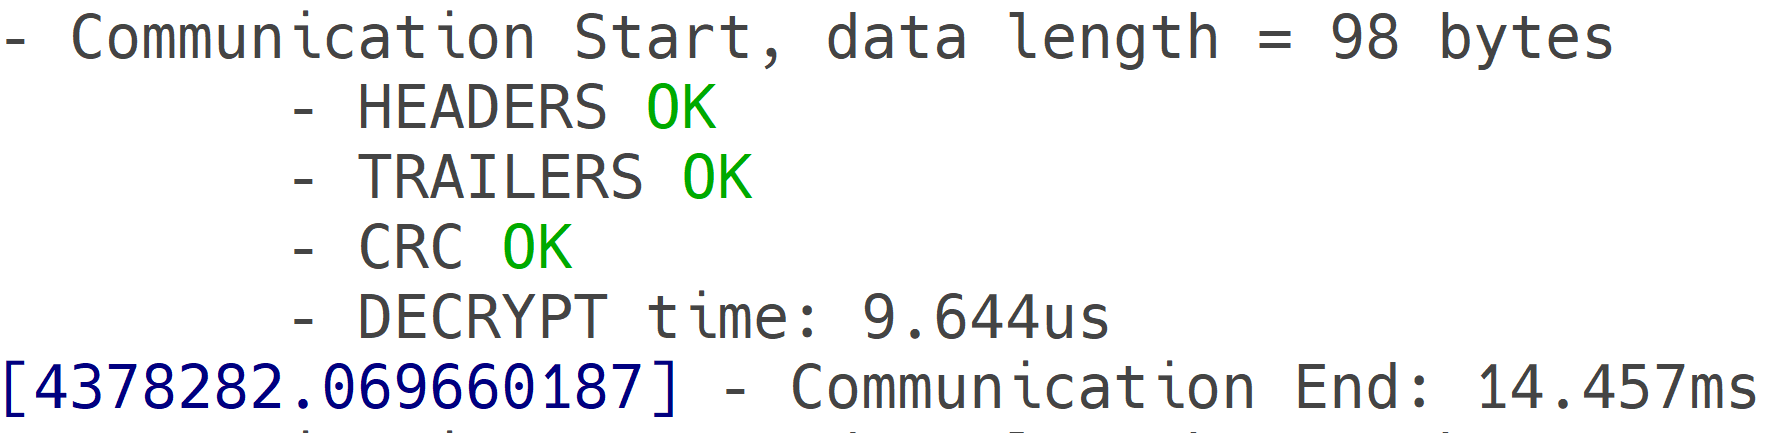
\includegraphics[width=1.0\linewidth, frame]{images/fig-frame-parsing-process-api-server.png}
\caption{Quá trình phân giải và xử lý cụ thể của một frame trên API server.}
\label{fig:frame-parsing-process-api-server}
\end{figure}

\begin{figure}[htp]
\centering
\captionsetup{justification=centering}
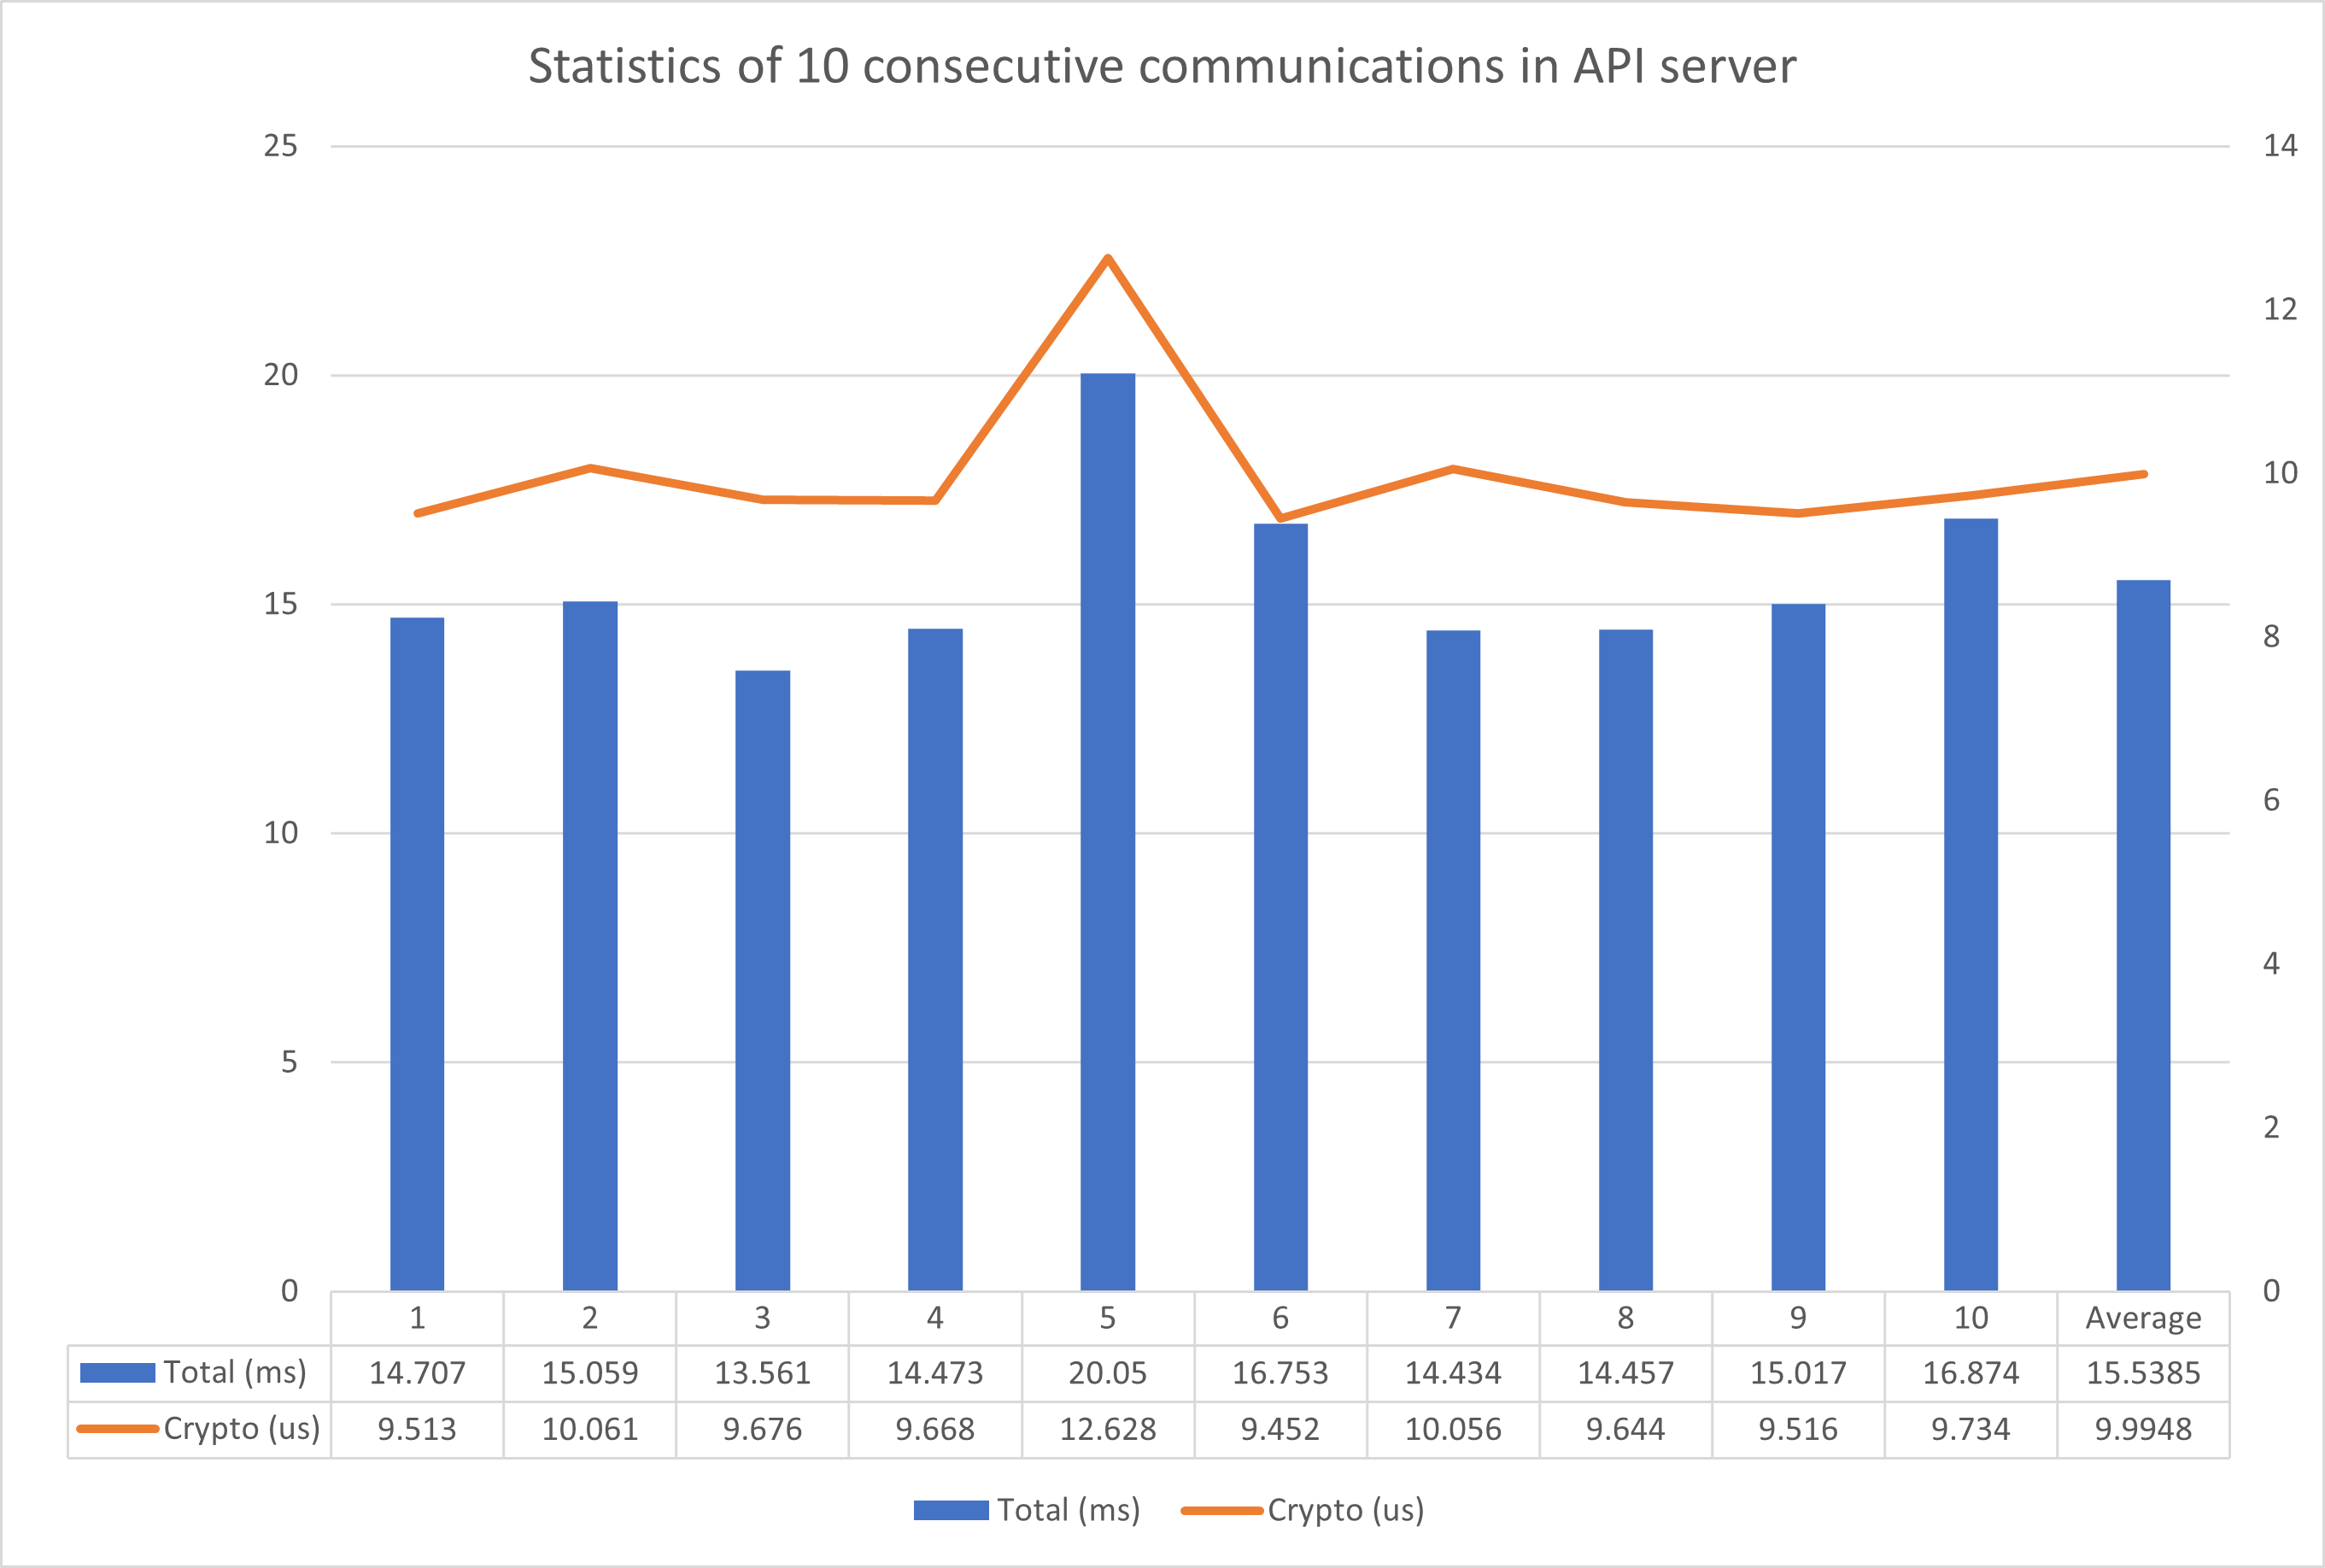
\includegraphics[width=1.0\linewidth, frame]{images/fig-10-measure-commu-server.png}
\caption{Thống kế của 10 quá trình giao tiếp liên tiếp với gateway trên API server.}
\label{fig:10-measure-commu-server}
\end{figure}

\subsection{Kết quả kỹ thuật mật mã hóa trên API server}

% Minh họa quá trình thiết lập key CC20, onetime key Poly1305
Kỹ thuật mật mã hóa sử dụng thuật toán \acrshort{aead} ChaCha20-Poly1305 được triển khai thành công trên \acrshort{api} server. Theo kiến trúc của thuật toán \acrshort{aead}, quá trình mã hóa (minh họa như hình \ref{fig:CC20-P1305-En-Process-server}) đã diễn ra đúng đắn và tuần tự theo các quá trình của RFC7539~\cite{rfc7539}:

\begin{enumerate}
    \item Thiết lập State cho Poly1305 one-time key.
    \item Tạo Poly1305 one-time key.
    \item Thực thi ChaCha20 encryption function.
    \item Thực thi Poly1305 function cho ciphertext.
\end{enumerate}

Và quá trình giải mã (minh họa như hình \ref{fig:CC20-P1305-De-Process-server}) đã diễn ra đúng đắn và tuần tự theo các quá trình của RFC7539~\cite{rfc7539}:

\begin{enumerate}
    \item Thiết lập State cho Poly1305 one-time key.
    \item Tạo Poly1305 one-time key.
    \item Thực thi Poly1305 function cho ciphertext.
    \item Thực thi ChaCha20 dencryption function.
\end{enumerate}

\begin{figure}[htp]
\centering
\captionsetup{justification=centering,margin=2cm}
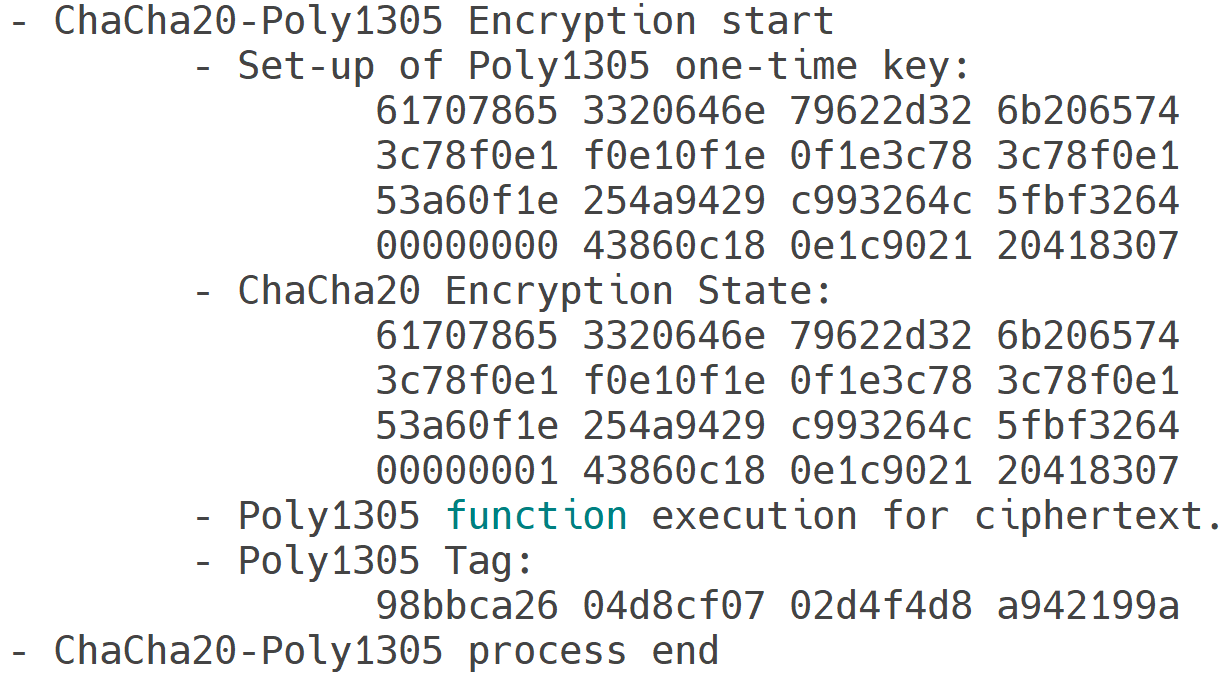
\includegraphics[width=0.7\linewidth, frame]{images/fig-CC20-P1305-En-Process-server.png}
\caption{Quá trình mã hóa của thuật toán \acrshort{aead} ChaCha20-Poly1305 trên API server.}
\label{fig:CC20-P1305-En-Process-server}
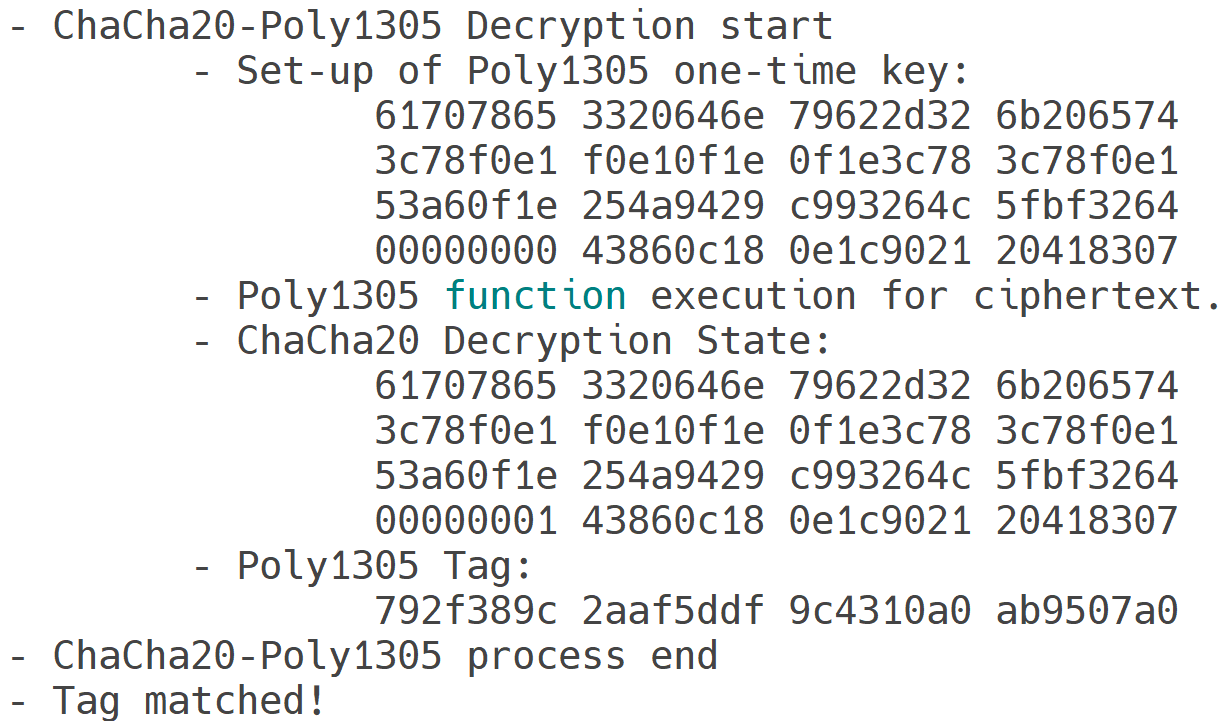
\includegraphics[width=0.7\linewidth, frame]{images/fig-CC20-P1305-De-Process-server.png}
\caption{Quá trình giải mã của thuật toán \acrshort{aead} ChaCha20-Poly1305 trên API server.}
\label{fig:CC20-P1305-De-Process-server}
\end{figure}

\subsection{Kết quả đồng bộ trên API server}

Kỹ thuật đồng bộ được triển khai thành công trên \acrshort{api} server. Trên công cụ Visual Studio Code, callback đồng bộ với model \acrshort{vs} (minh họa như hình \ref{fig:VS-callback-trig-server}) được thực hiện khi có sự thay đổi dữ liệu của \acrshort{vs} trên MongoDB database. Callback này được theo dõi thông qua breakpoint trên JavaScript Debug Terminal.

\begin{figure}[htp]
\centering
\captionsetup{justification=centering,margin=2cm}
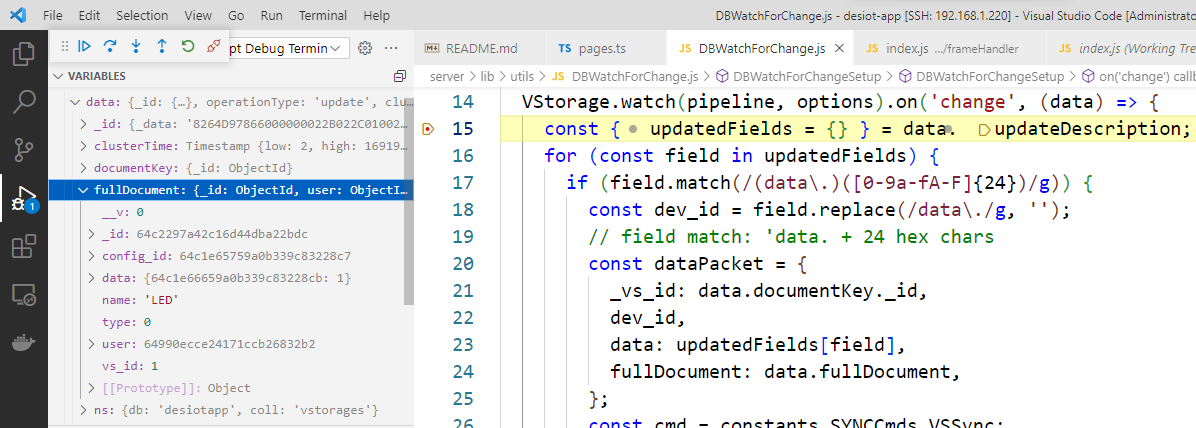
\includegraphics[width=1.0\linewidth, frame]{images/fig-VS-callback-trig-server.png}
\caption{Breakpoint theo dõi callback đồng bộ với \acrshort{vs} được thực hiện trên Visual Studio Code.}
\label{fig:VS-callback-trig-server}
\end{figure}

\section{Kết quả giao diện web}

Kết quả của giao diện web minh họa các kết nối với \acrshort{api} server, việc trực quan hóa dữ liệu của một thiết bị, và cấu hình \acrfull{pwa}.

\subsection{Kết nối với API server}

Giao diện web đã tổ chức thành công các kết nối với \acrshort{api} server. Cụ thể, khi truy cập vào giao diện của một thiết bị vật lý, network record của giao diện (minh họa như hình \ref{fig:network-fetch}) ghi lại các kết nối \acrshort{https} để lấy các dữ liệu khởi tạo và các kết nối Websocket để đồng bộ với sự thay đổi của các \acrshort{vs}. Trong đó, các kết nối \acrshort{https} (kiểu fetch) bao gồm:
\begin{itemize}
    \item \textbf{Current User}: lấy dữ liệu của người dùng hiện tại.
    \item \textbf{Device List}: lấy danh sách dữ liệu của tất cả thiết bị.
    \item \textbf{Current Device}: lấy dữ liệu của một thiết bị.
    \item \textbf{Current UI Dashboard}: lấy dữ liệu của một UI tab.
    \item \textbf{Get \acrlong{vs}}: lấy danh sách dữ liệu của tất cả \acrshort{vs}.
\end{itemize}

Và các kết nối Websocket (kiểu xhr) - \textbf{\acrshort{vs} Synchronization} bao gồm các request yêu cầu đồng bộ với sự kiện thay đổi dữ liệu các \acrshort{vs} trên \acrshort{api} server.

\begin{figure}[htp]
\centering
\captionsetup{justification=centering,margin=2cm}
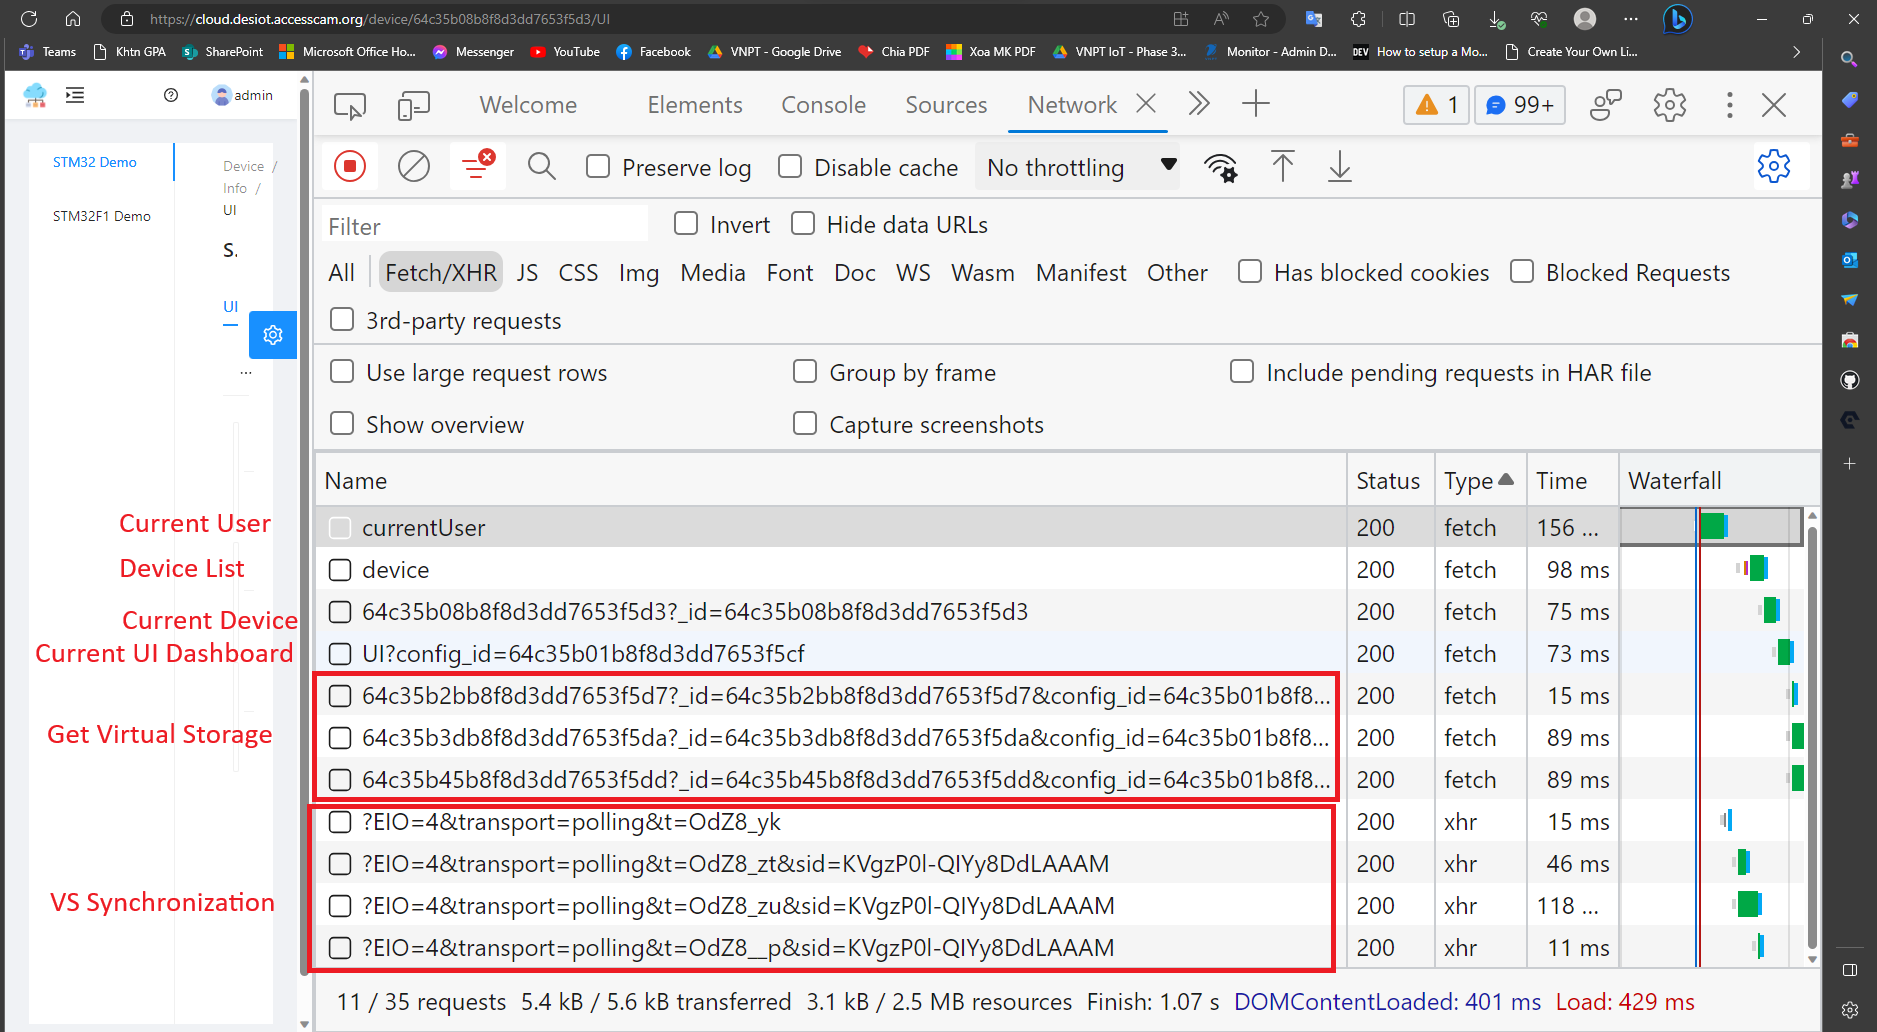
\includegraphics[width=1.0\linewidth, frame]{images/fig-network-fetch.png}
\caption{Các network record hiển thị các kết nối giao diện web và API server.}
\label{fig:network-fetch}
\end{figure}

\subsection{Trực quan hóa dữ liệu của thiết bị}

Trong việc trực quan hóa dữ liệu của một thiết bị, giao diện web đã hiển thị được các giá trị của database và hiển thị theo thay đổi thời gian thực. Cụ thể, giao diện web trực quan hóa dữ liệu phần cứng (minh họa như hình \ref{fig:web-interface-for-physic}), đã hiển thị dữ liệu phần cứng trên database thông qua các widget trên UI dashboard.

\begin{figure}[htp]
\centering
\captionsetup{justification=centering,margin=2cm}
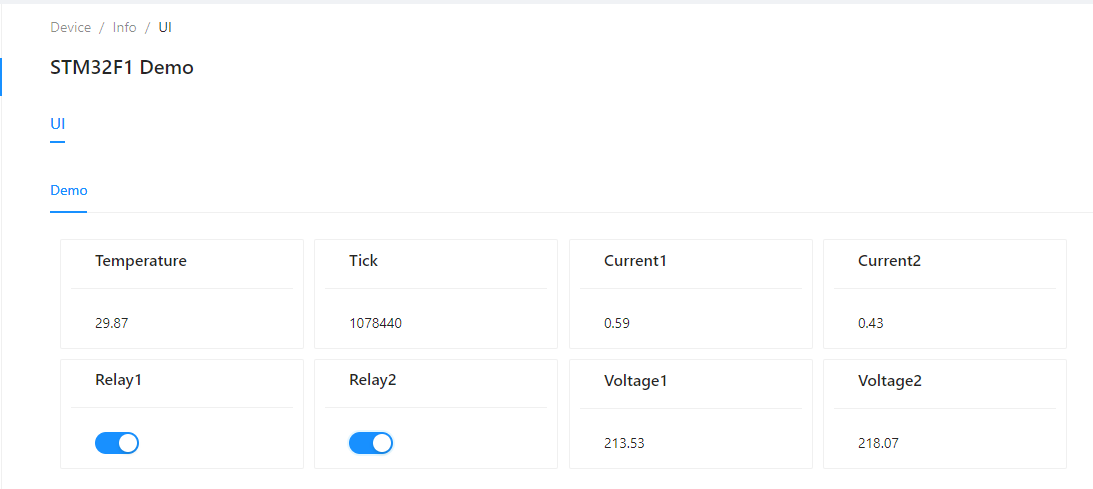
\includegraphics[width=1.0\linewidth, frame]{images/fig-web-interface-for-physic.png}
\caption{Giao diện web trực quan hóa dữ liệu phần cứng.}
\label{fig:web-interface-for-physic}
\end{figure}

Về việc hiển thị dữ liệu thời gian thực, các network record Websocket của giao diện web (minh họa như hình \ref{fig:websocket-records}) cho thấy dữ liệu phần cứng trên database luôn được đồng bộ real-time với các thành phần trên UI dashboard. Các record này được ghi lại thông qua Microsoft Edge Developer Tools.

\begin{figure}[htp]
\centering
\captionsetup{justification=centering,margin=2cm}
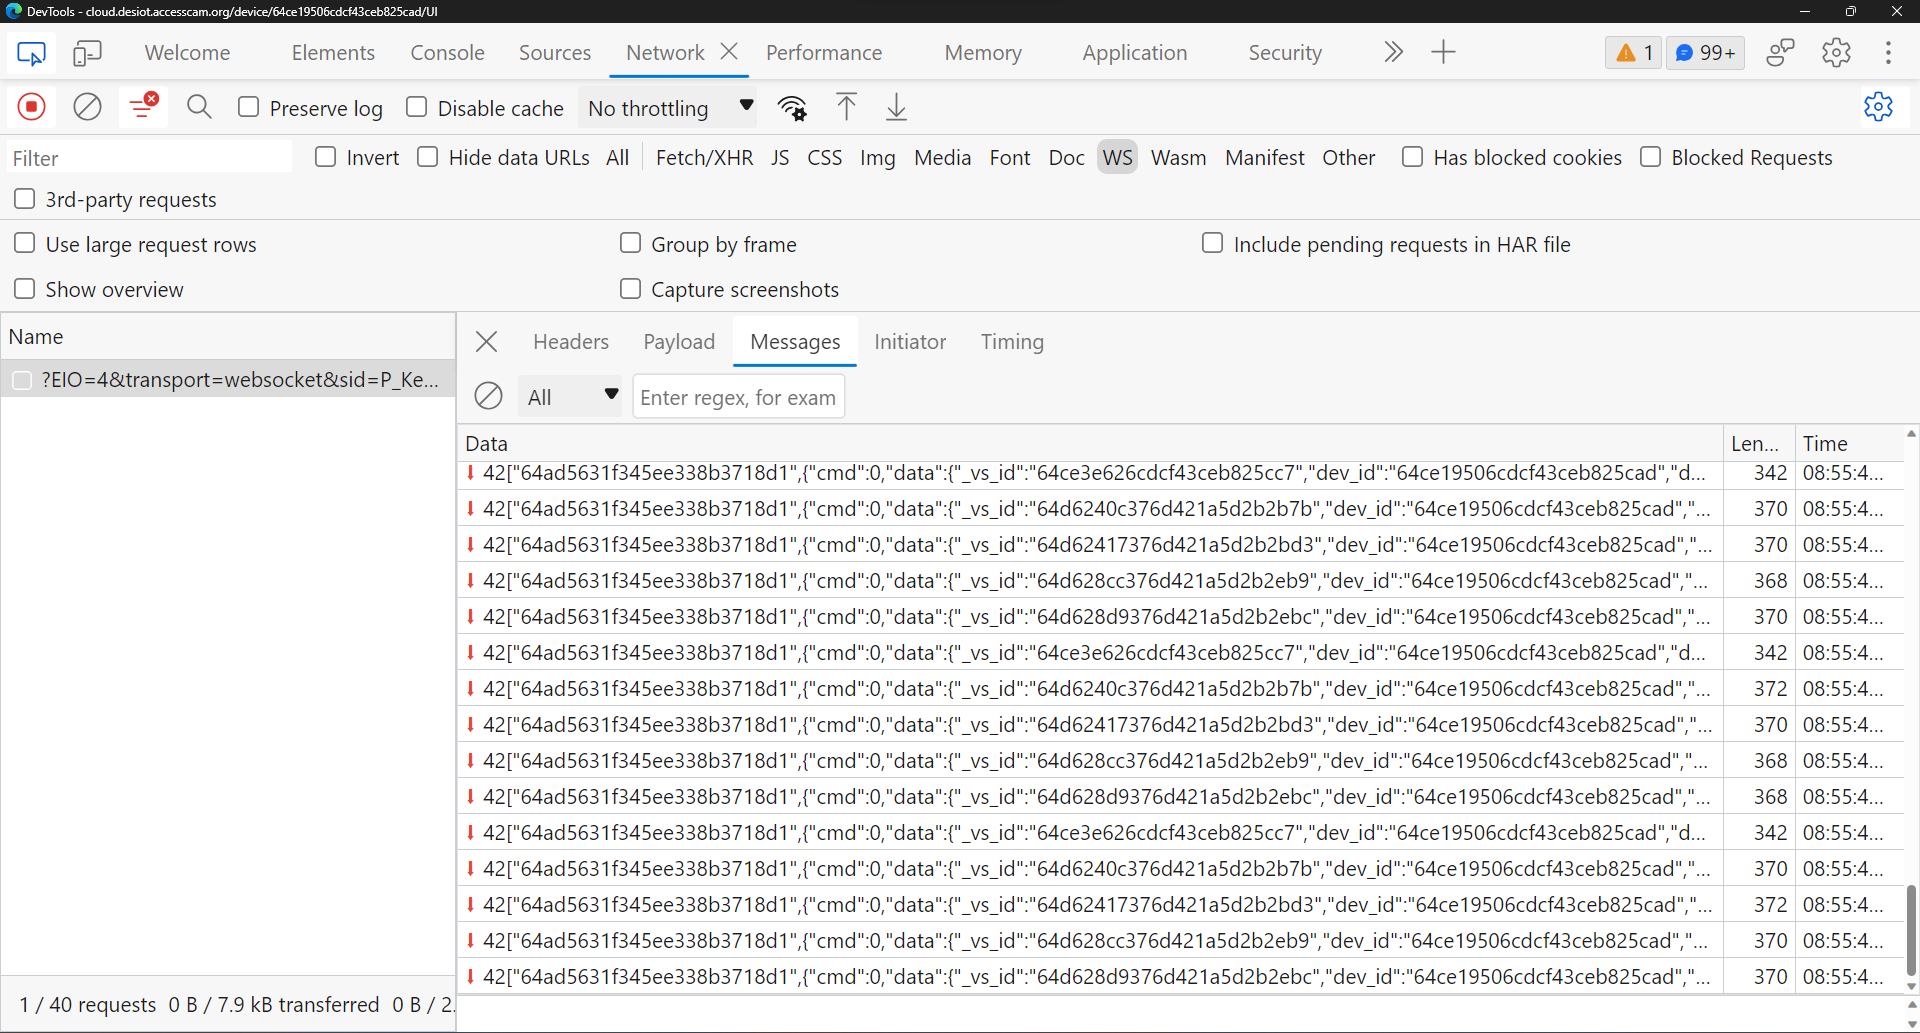
\includegraphics[width=1.0\linewidth, frame]{images/fig-websocket-records.png}
\caption{Các Websocket record trên giao diện web ghi lại thông qua Microsoft Edge Developer Tools.}
\label{fig:websocket-records}
\end{figure}

\subsection{Cấu hình PWA}

Cấu hình \acrshort{pwa} đã được triển khai trên giao diện web. Do đó, người dùng có thể cài đặt trang web như một ứng dụng trên nhiều nền tảng (desktop, mobile,...). Cụ thể, Lighthouse report (minh họa như hình \ref{fig:lighthouse-report}) đã chứng thực cấu hình \acrshort{pwa} của giao diện web.

\begin{figure}[htp]
\centering
\captionsetup{justification=centering,margin=2cm}
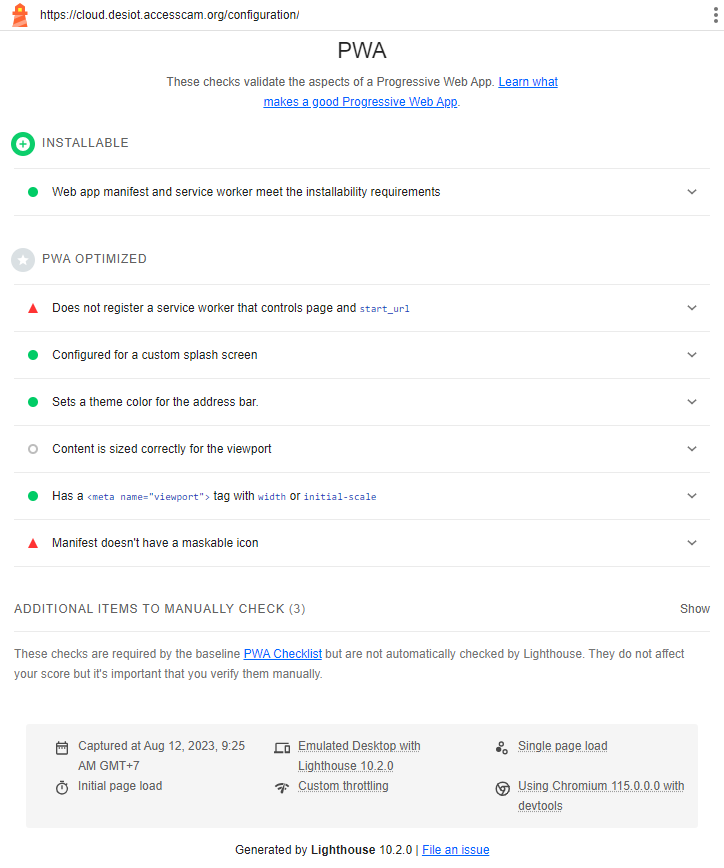
\includegraphics[width=1.0\linewidth, frame]{images/fig-lighthouse-report.png}
\caption{Lighthouse report của cấu hình PWA của giao diện web.}
\label{fig:lighthouse-report}
\end{figure}